\documentclass[paper=a4,fontsize=10pt]{jlreq}
\usepackage{amsmath,amsfonts,array,ascmac,amssymb} %数学に必要なパッケージ
\usepackage{tikz} %グラフ描画に必要なパッケージ
\usepackage{TeachersGuide}
\usetikzlibrary{calc}
\begin{document}
\showTitle{9月1日 1校時}{3年A組}{数学I}{数学I 数研出版}{溝口洸熙}
\unitTitle{二次関数「二次関数とそのグラフ」}
\begin{UnitGoals}
    \begin{itemize}
        \item 表,式,グラフなどを用いて数量の変化を表現することの有用性を認識し,関数の考えを具体的な事象の考察に活用しようとする.
        \item 関数の概念\dots
    \end{itemize}
\end{UnitGoals}
\begin{UnitView}
    \ \ 二次関数は,高校数学の中で最も基礎的であり,かつ重要な単元である.二次関数を扱い,関数概念の理解を深め,関数を用いて数量の変化を表現することの有用性を認識できるよう\dots
\end{UnitView}
\begin{EvaluationCriterion}
    \begin{enumerate}
        \enumiA
        \item 知識があるといいね
        \item 技能があるといいね
    \end{enumerate} &
    \begin{enumerate}
        \enumiB
        \item 思考があるといいね
        \item 判断があるといいね
        \item 表現があるといいね
    \end{enumerate} &
    \begin{enumerate}
        \enumiC
        \item 主体的に学習に取り組む態度があるといいね
    \end{enumerate}\\
    \hline
\end{EvaluationCriterion}
\begin{UnitPlan}
    第1時間目 & 関数の定義について学び,関数の値,値域を求める.& \fbox{A1},\fbox{B2} & 観察・小テスト・自己評価\\
    \hline
    第2時間目 & 関数のグラフの意味について学び,1時間数の最大値と最小値を求める.& \fbox{B1},\fbox{B2} & 観察・ワークシート\\
    \hline
    第3時間目 & 二次関数\(y=ax^2,y=ax^2+q\)のグラフを描く. & \fbox{A2},\fbox{B1} & 観察・ワークシート・自己評価\\
\end{UnitPlan}
\begin{StudentFacts}
    \ \ 中学校で習った一次関数\(y=ax+b\)や二次関数\(y=ax^2\)に対して苦手意識のある生徒が多く,グラフをかくことができない,関数とグラフの関係が分からないという生徒もいる.\par
    \ \ また,\dots
\end{StudentFacts}
\begin{ClassGoal}
    \begin{itemize}
        \item \(x\)軸方向へ平行移動する二次関数のグラフについて関心をもち,調べようとする.\fbox{C1}
        \item 二次関数 \(y=ax^2\)を\(x\)軸方向へ\(p\)だけ平行移動したグラフから二次関数の式を考察できる.\fbox{B1}
    \end{itemize}
\end{ClassGoal}
\begin{ClassPoint}
    \ \ 二次関数$y=a(x-p)^2$のグラフを考えるに当たって,先に式を与えてグラフをかかせることが一般的であるが,\dots
\end{ClassPoint}
\begin{TeachingProcedures}
    &
    \begin{tpbcol}
        \indent 半径\(r\)円の面積\(S\)の求め方を復習する.(\(S=\pi r^2\))\\
        \dotfill\\
        \indent ある曲線\(y=f(x)\)と\(x\)軸,及び2直線\(x=a\textrm{,}x=b\)で囲まれた部分の面積を求める方法を復習する.
    \end{tpbcol}& &
    \\
    & \begin{tpbcol}
        \begin{framed}
            \noindent\textbf{復習問題1}\par
            曲線\(y=\sqrt{x}\)と\(x\)軸,及び2直線\(x=1\textrm{,}x=2\)で囲まれた部分の面積を求めよ.
        \end{framed}
        \begin{framed}
            \begin{minipage}[c]{0.4\linewidth}
                \noindent\textbf{解答}(期待する解答)
                \begin{equation*}
                    \begin{aligned}
                        S & =\int_{1}^{2}\sqrt{x}\quad dx                      \\
                          & = \left[\dfrac{2}{3}x^{\frac{3}{2}}\right]^{2}_{1} \\
                          & = \dfrac{2}{3}\cdot 2^{\frac{3}{2}}-\dfrac{2}{3}   \\
                          & =\dfrac{2}{3}\left(2\sqrt{2}-1\right)
                    \end{aligned}
                \end{equation*}
            \end{minipage}
            \begin{minipage}[c]{0.56\linewidth}
                \centering
                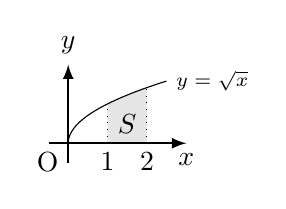
\begin{tikzpicture}[samples=300,scale=0.5]
                    \fill[fill=gray!20] plot[domain=1:2](\x, {sqrt(\x)})--(2,0)--(1,0)--cycle;
                    \draw[-latex,thick](-0.5,0)--(3,0)node[below]{\(x\)};
                    \draw[-latex,thick](0,-0.5)--(0,2)node[above]{\(y\)};
                    \node[below left] at(0,0){O};
                    \draw[domain=0:2.5] plot(\x, {sqrt(\x)})node[right]{\scriptsize \(y=\sqrt{x}\)};
                    \node at ($(2,0)!0.5!(1,1)$){\(S\)};
                    \draw[dotted](1,0)node[below]{1}--(1,1);
                    \draw[dotted](2,0)node[below]{2}--(2,{sqrt(2)});
                \end{tikzpicture}
            \end{minipage}
        \end{framed}
    \end{tpbcol} &
    \begin{tpccol}
    \end{tpccol} &
    \begin{tpdcol}
    \end{tpdcol}\\
    \hline
    &
    \begin{tpbcol}
        \textbf{回転体(具体例)}\\
        \indent\(a<b\)のとき,曲線\(y=\sqrt{x}\)と\(x\)軸,及び2直線\(x=1\textrm{,}x=2\)で囲まれた部分を,\(x\)軸の周りに1回転させてできる立体の体積\(V\)を考える.\par
        \indent ある\(x\)軸上の点A\((1,0)\)で考える.\underline{半径}に着目して,断面積を求めたい.\(x\)軸上の点\((x',0)\)の断面積は,\((\sqrt{x'})^2\times \pi\)で求めることができる.\\
        \indent 従って,断面積を\(S(x)\)とすると,\(S(x)=\pi(\sqrt{x})^2\)となる.回転体の面積を求めるためには,\(1\leqq x \leqq 2\)の範囲で\(S(x)\)を求める必要があるので,\(S(x)\)を\(1\leqq x \leqq 2\)の範囲で\(x\)について積分して,回転体の面積を求める.つまり,
        \begin{equation}
            \begin{aligned}
                V & = \int_{1}^{2} S(x) dx                            \\
                  & = \pi\int_{1}^{2} \big\{\sqrt{x}\big\}^2 dx = \pi
            \end{aligned}
        \end{equation}
        で求めることができる.
    \end{tpbcol} &
    \begin{tpccol}
        \textbf{黒板にグラフを描画して考えるように促す}
        \begin{center}
            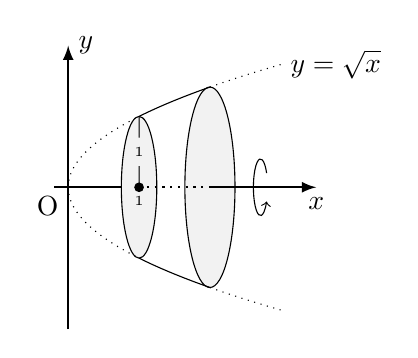
\begin{tikzpicture}[samples=300,scale=0.9]
                \def\Fx{plot(\x,{sqrt(\x)})};
                \def\dFx{plot(\x,{-1*sqrt(\x)})};
                \filldraw[draw=black,fill=gray!10](2,0)ellipse({sqrt(2)/4} and {sqrt(2)});
                \filldraw[draw=black,fill=gray!10](1,0)ellipse({sqrt(1)/4} and {sqrt(1)});
                \draw[domain=1:2] \Fx \dFx;
                \draw[domain=2:3,dotted] \Fx node[right]{\(y=\sqrt{x}\)} \dFx;
                \draw[domain=0:1,dotted] \Fx \dFx;
                \draw[thick](-0.2,0)--(0.75,0);
                \draw[thick,dotted](1,0)--(2,0);
                \draw[-latex,thick](2,0)--(3.5,0)node[below]{\(x\)};
                \draw[-latex,thick](0,-2)--(0,2)node[right]{\(y\)};
                \node[below left] at (0,0){O};
                \draw[->](2.8,0.2)arc[start angle=30, end angle=330, x radius=0.1, y radius=0.4];
                \node at (1,1/2)(r){\tiny 1};
                \draw[thin,fill=black](1,0)circle[radius=0.06]node[below]{\tiny 1}--(r)--(1,1);
            \end{tikzpicture}
            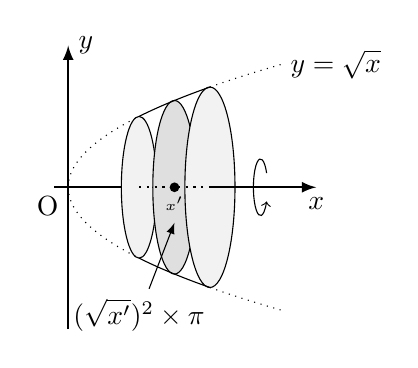
\begin{tikzpicture}[samples=300,scale=0.9]
                \def\Fx{plot(\x,{sqrt(\x)})};
                \def\dFx{plot(\x,{-1*sqrt(\x)})};
                \filldraw[draw=black,fill=gray!10](1,0)ellipse({sqrt(1)/4} and {sqrt(1)});
                \filldraw[draw=black,fill=gray!25](1.5,0)ellipse({sqrt(1.5)/4} and {sqrt(1.5)});
                \filldraw[draw=black,fill=gray!10](2,0)ellipse({sqrt(2)/4} and {sqrt(2)});
                \draw[domain=1:2] \Fx \dFx;
                \draw[domain=2:3,dotted] \Fx node[right]{\(y=\sqrt{x}\)} \dFx;
                \draw[domain=0:1,dotted] \Fx \dFx;
                \draw[thick](-0.2,0)--(0.75,0);
                \draw[thick,dotted](1,0)--(2,0);
                \draw[-latex,thick](2,0)--(3.5,0)node[below]{\(x\)};
                \draw[-latex,thick](0,-2)--(0,2)node[right]{\(y\)};
                \node[below left] at (0,0){O};
                \draw[->](2.8,0.2)arc[start angle=30, end angle=330, x radius=0.1, y radius=0.4];
                \draw[fill=black](1.5,0)circle[radius=0.06]node[below]{\tiny \(x'\)};
                \node at (1,-1.8)(s) {\((\sqrt{x'})^2\times \pi\)};
                \draw[-latex](s)--(1.5,-0.5);
            \end{tikzpicture} \\
        \end{center}
    \end{tpccol} &
    \begin{tpdcol}
    \end{tpdcol} \\
    &
    \begin{tpbcol}
        \textbf{一般化}\par
        \indent 一般的に,曲線\(y=f(x)\)と\(x\)軸,及び2直線\(x=a\textrm{,}x=b (a<b)\)で囲まれた部分を,\(x\)軸の周りに1回転させてできる立体の体積を\(V\)とすると,以下の公式が得られる.
        \begin{equation}
            \begin{aligned}
                V = \pi\int_{a}^{b}\big\{f(x)\big\}^2dx = \pi\int_{a}^{b}y^2dx
            \end{aligned}
        \end{equation}
        \begin{flushright}
            \((a<b)\)
        \end{flushright}
    \end{tpbcol} &
    \begin{tpccol}

    \end{tpccol} &
    \begin{tpdcol}

    \end{tpdcol}\\
    \hline
    &
    \begin{tpbcol}
        \textbf{例題5}\\
        \indent この例題を用いて,教科書を見ながら一度解き方を確認する.
        \begin{itemize}
            \setlength{\leftskip}{-1em}
            \item \(\cos ^2 x\)の積分を確認をする.
        \end{itemize}
        \dotfill
    \end{tpbcol} &
    \begin{tpccol}
        \textbf{問題のすすめ方}\\
        \indent 実際にグラフを描いて,教科書に沿った方法で説明する.そして,他の解法を思いついた生徒には挙手させ,説明させる.その解法が正解かどうかをみんなで議論する.\\
        \dotfill
    \end{tpccol} &
    \begin{tpdcol}

    \end{tpdcol}\\
    &
    \begin{tpbcol}
        \textbf{問題8}\\
        \indent 15分間で,(1),(2)を解く.
    \end{tpbcol} &
    \begin{tpccol}
        \textbf{問題のすすめ方}\\
        \indent グラフを書くように促す.
    \end{tpccol} &
    \begin{tpdcol}

    \end{tpdcol}\\
\end{TeachingProcedures}
\end{document}